\addcontentsline{toc}{subsection}{Compilación histórica del estudio astronómico}
\subsection*{Compilación histórica del estudio astronómico}
El estudio de los movimientos celestes ha sido una de las áreas fundamentales de la astronomía desde la antigüedad. 
Las civilizaciones mesopotámica, egipcia y maya registraron observaciones detalladas de la Luna y sus fases, utilizándolas para
la medición del tiempo y la elaboración de calendarios lunares \cite{antigua}.

La antigua civilización Maya, tenía conocimiento de la importancia y complejidad de la información
astronómica y calendárica. Esto indica que existía un contexto interpretativo especialmente prometedor que se 
fortaleció aun más tras la escritura jeroglífica proporcionando conocimiento clave del cielo y su aplicación social. Este conocimiento también
se reflejaba en un complejo sistema de contar meses lunares asociados a fechas escritas en la llamada cuenta larga que usaban para calcular y representar
el tiempo y pronto se dieron cuenta que podía servir para cálculos astronómicos \cite{maya}.


\begin{figure}[h]
    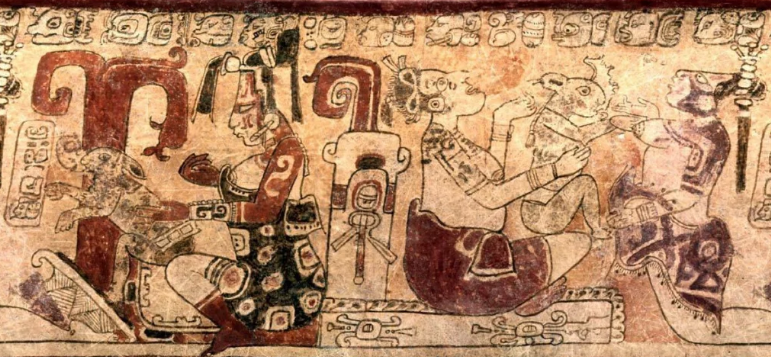
\includegraphics[scale = 0.7]{Imagenes/MayasMoon.png}
    \centering
    \caption{Puerta tallada de la diosa lunar Maya}{Fuente: Adaptado de \cite{ixchel}}
\end{figure}


Con el desarrollo del método científico, un gran exponente es Galileo Galilei quien es el precursor de la cosmología moderna ya que establecía
leyes sistemáticas capaces de ser observadas y expresadas en un lenguaje físico-matemático. Galileo mejoró el telescopio de la época y en sus observaciones
que son descritas en su libro "Sidereus Nuncius" \cite{sidereus} en 1610 establece que la Vía Láctea está compuesta por innumerables estrellas asociadas en complejos sistemas. En este texto se encuentran sus famosas observaciones telescópicas de la superficie lunar
y su anuncio del descubrimiento de cuatro satélites de Júpiter
(Ío, Europa, Ganímedes y Calixto), denominados por Galileo
“astros mediceos”


\begin{figure}[h]
    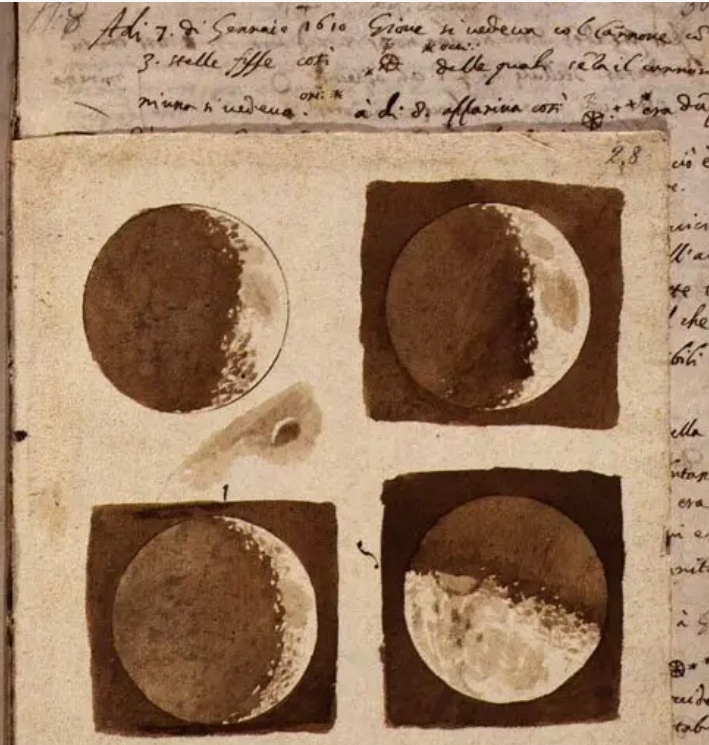
\includegraphics[scale = 0.5]{Imagenes/GalileoMoon.png}
    \centering
    \caption{Primeros dibujos de la Luna realizados por Galileo Galilei}{ Adaptado de: \cite{bbc}}

\end{figure}

\addcontentsline{toc}{subsection}{Historia de la simulación en la astronomía}
\subsection*{Historia de la simulación en la astronomía}

Los primeros modelos y representaciones que se tenían sobre la representación 
de fenomenos astronómicos se pueden encontrar en el papiro "Liber de coelo et mundo"
donde se aprecian diagramas geométricos relacionados con círculos y diámetros lo que da a entender
que el contenido estaba relacionado con astronomía y geometría esférica.

\begin{figure}[H]
    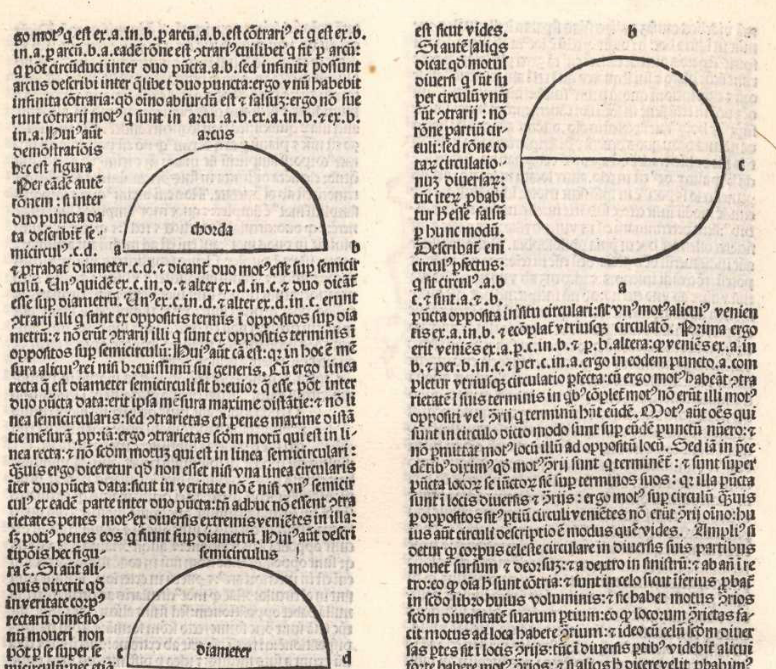
\includegraphics[scale = 0.55]{Imagenes/papiro.png}
    \centering
    \caption{Representación geométrica de cuerpos celestes}{ Adaptado de: \cite{decaelo}}
\end{figure}

También se destaca una curiosa representación de las fases de la luna en el año 1492 del capítulo `Liber de coelo et mundo' del libro `Introductiones in Aristotelis libros naturales' del teólogo francés y erudito griego Jacques Lefèvre d'Étaples.

\begin{figure}[H]
    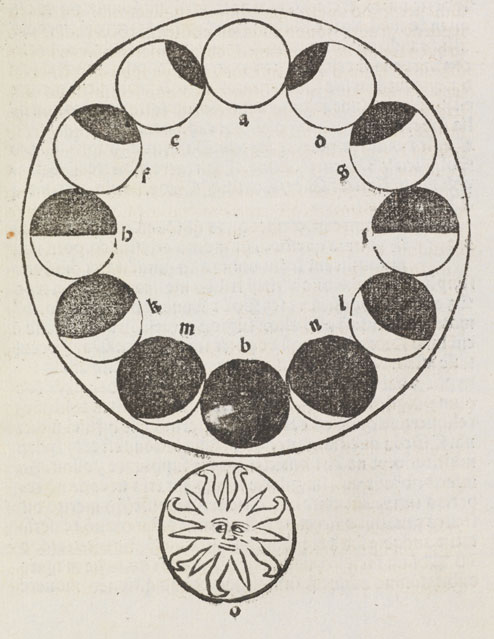
\includegraphics[width = 12cm, height=7.5cm]{Imagenes/fasesLunares1492.png}
    \centering
    \caption{Fases Lunares de Itroductiones in Aristotelis libros naturales}{ Adaptado de: \cite{lunarspine}}
\end{figure}
